\documentclass{scrartcl}
\usepackage{mm_ws15}

\newcommand{\sheetTitle}{Blatt 10, Abgabe 12.1.2016} 
\begin{document}
\maketitle


%%%%%%%%%%%%%%%%%%%%%%%%%%%%%%%%%%%%%%%%%%%%%%%%%%%%%%%%%%%%%%%%%%%%%%%%%%%%%%%%
\section{Fadenpendel \points{12}}
\label{sec:fadenpendel}

Ein Massepunkt der Masse $m$ befindet sich an einem Ende eines starren, masselosen \quotes{Faden} der Länge $l$, dessen anderes Ende in einem Punkt fixiert ist.
Die Differentialgleichung für die Bewegung des Massepunktes im Schwerefeld der Erde lautet
\[
  ml \frac{\dd^2 \phi}{\dd t^2}(t) = - m g \sin \phi(t).
  \label{eq:faden}
\]
Hierbei bezeichnet $\phi \in [-\pi, \pi]$ den Auslenkwinkel aus der Ruhelage.
\begin{subex}
  \item\points{3} Fertigen Sie eine Skizze des Pendels an und nutzen Sie diese, um die Bewegungsgleichung herzuleiten.
  \item\points{1} Da die Differentialgleichung~\eqref{eq:faden} nicht elementar lösbar ist, verwenden wir die Kleinwinkelnäherung für kleine Auslenkungen $\phi$:
  \[
    \sin \phi \approx \phi.
  \]
  Begründen Sie diese.
  \item\points{2} Finden Sie die allgemeine Lösung von~\eqref{eq:faden} unter der Kleinwinkelnäherung.
  \item\points{2} Man kann die genäherte Gleichung in der Form $\mathcal{L}\phi = 0$ schreiben, wobei $\mathcal{L}$ ein linearer Differentialoperator ist. 
  Was folgt daraus für Lösungen $\phi_1(t)$ und $\phi_2(t)$ der genäherten Gleichung?
  Gilt die selbe Aussage auch für Lösungen von~\eqref{eq:faden}?  
  Geben Sie $\mathcal{L}$ explizit an.
  \item\points{4} Wie lautet die Lösung, falls das Pendel zum Zeitpunkt $t = 0$ um $\phi_0$ ausgelenkt wurde und die Anfangsgeschwindigkeit $\frac{\dd \phi}{\dd t}(0) = 0$ ist?
  Berechnen Sie die Periodendauer, d.h.\ die kleinste Zeit $T > 0$, bei der erneut $\phi(t) = \phi_0$ gilt.
\end{subex}

\newpage
%%%%%%%%%%%%%%%%%%%%%%%%%%%%%%%%%%%%%%%%%%%%%%%%%%%%%%%%%%%%%%%%%%%%%%%%%%%%%%%%
\section{Wellengleichung in einer Dimension \points{18}}
\label{sec:wellengleichung_in_einer_dimension}

Wellengleichungen gehören zu den wichtigsten partiellen Differentialgleichungen in der Physik.
In dieser Aufgabe sollen Sie die Wellengleichung aus einem einfachen Model herleiten und ihre allgemeine Lösung bestimmen.

\begin{subex}
  \item\points{4} Wir betrachten eine endliche, lineare Kette (siehe Skizze) als Model für ein eindimensionales Medium, in dem sich die Welle ausbreitet:
  Die Kette besteht aus $N$ Massepunkten der Masse $m$, die über ideale Federn mit Federkonstante $k$ verbunden sind.
  In Ruhelage haben die Massen den Abstand $h$.
  Wir betrachten nur longitudinale Auslenkungen, d.h. Abweichungen von der Ruhelage \emph{entlang} der Kette.
  Die \emph{Auslenkung} der $i$-ten Masse aus ihrer Ruhelage zum Zeitpunkt $t$ beschreiben wir durch die Variable $\varphi_i(t)$.

  Nach dem Hookschen Gesetz ist die Rückstellkraft einer Feder proportional zu ihrer Ausdehnung oder Stauchung $\Delta x$ und wirkt dieser entgegen:
  \[
    F_{\mathrm{H}} = -k \Delta x.
  \]
  Leiten Sie aus den Newtonschen Gesetzen die Bewegungsgleichung für die Auslenkung der $i$-ten Masse her:
  \[
    m \frac{\dd^2 \varphi_i}{\dd t^2} (t) = k \left[ \varphi_{i+1}(t) - 2 \varphi_i(t) + \varphi_{i-1}(t) \right].
  \]
  Klassifizieren Sie diese Differentialgleichungen.


  \item\points{4} Zur Beschreibung eines kontinuierlichen Systems (z.B.\ eines elastischen Gummibands) betrachten wir nun den Grenzfall $N \to \infty$, wobei die Gesamtlänge $L = Nh$, die Gesamtmasse $M = Nm$, sowie $K = k/N$ konstant bleiben sollen.
  Die longitudinale Auslenkung zur Zeit $t$ eines Punktes mit Ruhelage $x$ wird dann beschrieben durch $\varphi(x, t)$.
  Für den diskreten Fall heißt das $\varphi_i(t) = \varphi(x=i h, t)$.

  Zeigen Sie, dass die Bewegungsgleichung im kontinuierlichen Grenzfall die Form
  \[
    \frac{\partial^2}{\partial t^2} \varphi(x, t) = c^2 \frac{\partial^2}{\partial x^2} \varphi(x, t)
    \label{eq:eom}
  \]
  hat.
  Bestimmen Sie die Konstante $c^2$ aus den Parametern des diskreten Modells $L$, $M$ und $K$.
  \begin{remark}{Hinweis}
    Zeigen Sie, dass sich die zweite Ableitung einer Funktion $f(x)$ durch folgenden Grenzwert ausdrücken lassen:
    \[
      \frac{\dd^2 f}{\dd x^2}(x) = \lim_{h \to 0} \frac{f(x + h) - 2f(x) + f(x - h)}{h^2}
    \] 
    
  \end{remark}


  \item\points{6} In der Vorlesung wurde die allgemeine Lösung für die sogenannten Dirichlet-Randbedingungen $\varphi(0, 0) = \varphi(L, 0) = 0$ 
  \[
    \varphi(x, t) = \Re \left( \sum_{k=1}^\infty C_k \sin \left( \frac{k\pi}{L} x \right) \ee^{\ii c \frac{k\pi}{L} t} \right)
  \]
  mithilfe des Separationsansatzes hergeleitet.
  Leiten Sie analog die allgemeine Lösung für sogenannte von Neumann-Randbedingungen 
  \[
    \pderiv[\varphi]{x}(0, t) = \pderiv[\varphi]{x}(L, t) = 0
    \label{eq:neumann}
  \]
  her.
  Lösen Sie mit Hilfe dieser das Anfangswertproblem
  \[
    \varphi(x, 0) = \cos\left(\frac{\pi x}{L}\right) + \frac{1}{10} \cos\left( \frac{2\pi x}{L} \right).
  \]
  \begin{remark}{Bemerkung}
    Die von Neumann-Randbedingungen werden auch offene Randbedingungen genannt und treten u.a.\ bei transversalen Schwingungen auf:
    Angenommen eine Saite ist entlang der $x$-Achse gespannt; bezeichne die Auslenkung der Saite in $y$-Richtung an der Position $x$ zur Zeit $t$ mit $\varphi(x, t)$.
    Die Zeitentwicklung von $\varphi$ kann näherungsweise auch durch eine Wellengleichung beschrieben werden.
    Die Randbedingungen~\eqref{eq:neumann} gelten für eine Saite, die so eingespannt ist, dass ihre Aufhängepunkte sich frei in $y$-Richtung bewegen können.
  \end{remark}


  \item\points{4} Zeigen Sie, dass die Überlagerung einer links- und einer rechtslaufenden Welle
  \[
    \varphi(x, t) = \sin\left( \frac{\pi}{L} (x + ct) \right) + \sin\left( \frac{\pi}{L} (x - ct) \right)
  \]
  eine Lösung der Wellengleichung mit Dirichlet-Randbedingungen ist.
  Skizzieren Sie $\varphi(x, t)$ für die Zeiten $t_1 = 0$, $t_2 = \frac{L}{2c}$ und $t_3 = \frac{L}{c}$ und beschreiben Sie die Zeitentwicklung dieser Lösung.
\end{subex}

\begin{figure}[htbp]
  \centering
  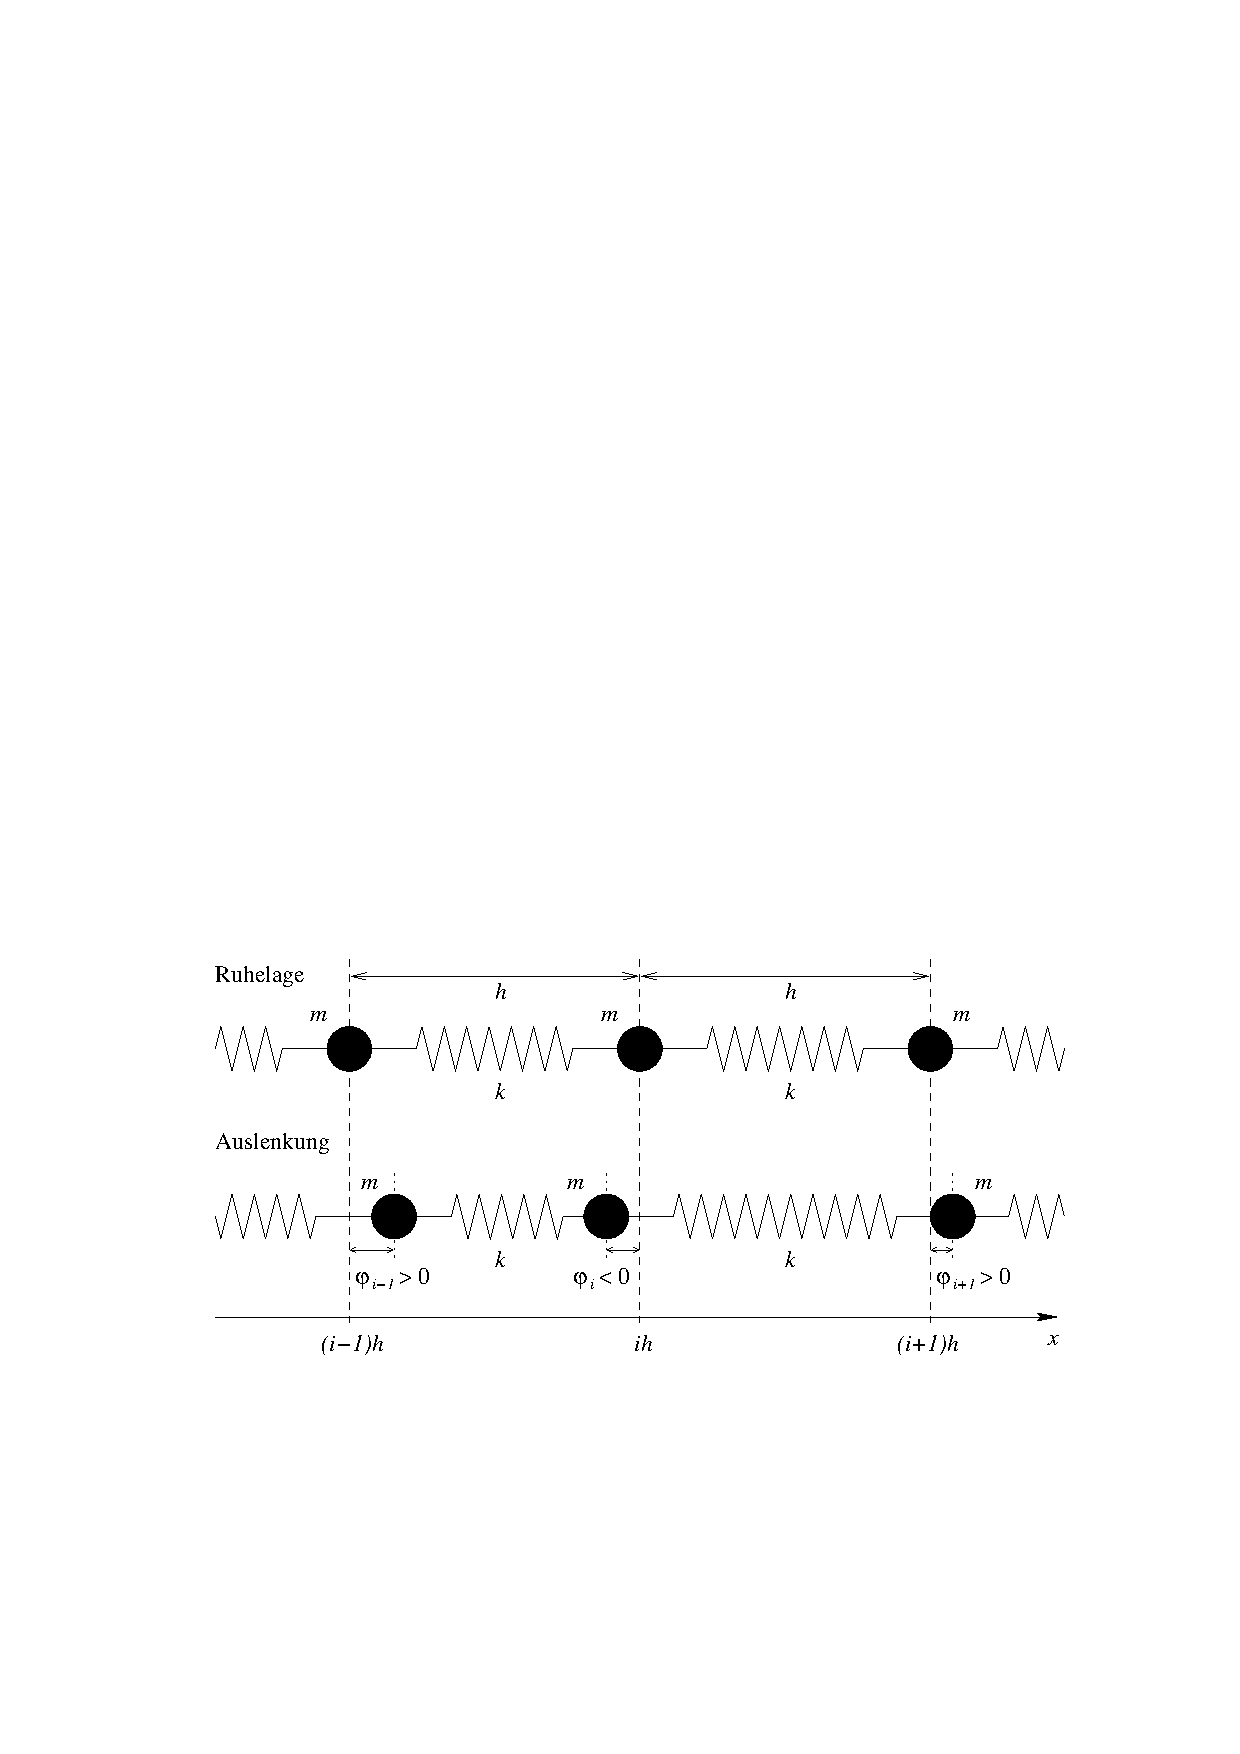
\includegraphics[width=0.95\textwidth]{img/chain}
\end{figure}
\end{document}
